\documentclass{beamer}
\usepackage[latin1]{inputenc}
\usepackage{xcolor}
\usepackage{hyperref}
\usepackage{minted}
\usepackage{tikz}
\usepackage{graphicx}

\usetheme{default}
\usecolortheme{default}

\title{COMP3320 Introduction to OpenGL}
\author{Alex Biddulph}
\institute{
    The University of Newcastle, Australia
    \and
    Based on the work provided at \url{www.learnopengl.com}
}
\date{Semester 2, 2019}

\begin{document}

\begin{frame}
\titlepage
\end{frame}

\begin{frame}{OpenGL Coordinates}
    \begin{itemize}
        \item OpenGL uses a right-handed coordinate system
        \item OpenGL uses normalised device coordinates
        \item[]
        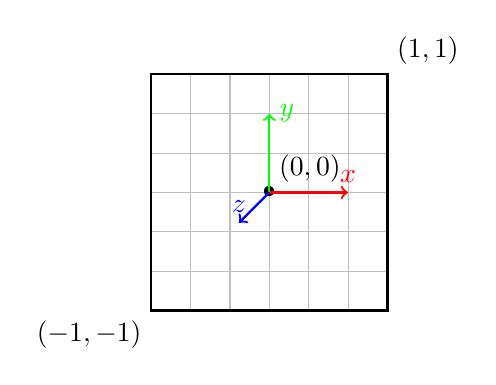
\begin{tikzpicture}[baseline={([yshift=-1em] current bounding box.north)}]
            % Grid lines
            \draw[step=0.5,lightgray,thin] (-1.5, -1.5) grid (1.5, 1.5);

            % Window edges
            \draw[thick] (-1.5, -1.5) -- (-1.5, 1.5) -- (1.5, 1.5) -- (1.5, -1.5) -- cycle;

            % Coordinates
            \draw (-1.5, -1.5) node[below left]{$\left(-1, -1\right)$};
            \draw (1.5, 1.5) node[above right]{$\left(1, 1\right)$};
            \draw (0, 0) node{\textbullet};
            \draw (0, 0) node[above right]{$\left(0, 0\right)$};

            % The axes
            \draw[thick,red,->]   (xyz cs:x=0.0) -- (xyz cs:x=1.0) node[above] {$x$};
            \draw[thick,green,->] (xyz cs:y=0.0) -- (xyz cs:y=1.0) node[right] {$y$};
            \draw[thick,blue,->]  (xyz cs:z=0.0) -- (xyz cs:z=1.0) node[above] {$z$};
        \end{tikzpicture}
        \item OpenGL will map the normalised device coordinates to the viewport dimensions
        \begin{itemize}
            \item $\left(-1, -1\right) \to \left(0, 0\right)$
            \item $\left(1, 1\right) \to \left(800, 600\right)$
        \end{itemize}
    \end{itemize}
\end{frame}

\begin{frame}{OpenGL Shaders}
    \begin{figure}
        \includegraphics{images/pipeline.png}
        \caption{Graphics pipeline stages.}
    \end{figure}
    \vfill{}
    Image sourced from \url{learnopengl.com/Getting-started/Hello-Triangle}
\end{frame}

\begin{frame}{OpenGL Shaders}
    \begin{itemize}
        \item Vertex Data: A list of 3D vertex coordinates and associated vertex attributes
        \item Vertex Shader: Transforms vertex coordinates from model space to clip space
        \item Shape Assembly: Assembles transformed vertices into a given primitive shape (e.g. triangles)
        \item Geometry Shader: Transforms shape geometry by emitting new vertices
        \item Rasterization: Maps primitives to pixel space and creates fragments
        \item Fragment Shader: Calculates the final colour for a pixel
        \item Tests and Blending: Performs depth testing and alpha blending
    \end{itemize}
\end{frame}

\begin{frame}[fragile]{OpenGL Shaders}
    \begin{itemize}
        \item Written in OpenGL Shader Language (GLSL)
        \item A simple vertex shader
\begin{minted}{glsl}
#version 330 core
layout (location = 0) in vec3 aPosition;
void main() { gl_Position = vec4(aPosition, 1.0); }
\end{minted}
        \item A simple fragment shader
\begin{minted}{glsl}
#version 330 core
out vec4 FragColour;
void main() {
    FragColour = vec4(1.0f, 0.5f, 0.2f, 1.0f);
}
\end{minted}
        \item Create a shader using {\color{blue}\verb"glCreateShader"}
        \item Attach shader source code using {\color{blue}\verb"glShaderSource"}
        \item Compile a shader using {\color{blue}\verb"glCompileShader"}
    \end{itemize}
\end{frame}

\begin{frame}[fragile]{OpenGL Shader Programs}
    \begin{itemize}
        \item Consists of multiple OpenGL shaders
        \begin{itemize}
            \item If you have a vertex shader, you must have a fragment shader
            \item If you have a fragment shader, you must have a vertex shader
            \item Geometry shader is optional
        \end{itemize}
        \item Create a shader program using {\color{blue}\verb"glCreateProgram"}
        \item Attach shaders to the program using {\color{blue}\verb"glAttachShader"}
        \item Link attached shaders together into the final program using {\color{blue}\verb"glLinkProgram"}
        \item Make a shader program active by using {\color{blue}\verb"glUseProgram"}
    \end{itemize}
\end{frame}

\begin{frame}[fragile]{Vertex Buffer Objects}
    \begin{itemize}
        \item Stores vertex data in GPU memory
        \item To create a vertex buffer use {\color{blue}\verb"glGenBuffers"}
        \item Program could consist of multiple different vertex buffers. To make a vertex buffer active use
            {\color{blue}\verb"glBindBuffer"}
        \item Vertex data is defined as a list of 3D coordinates (and optionally vertex attributes)
 \begin{minted}{c++}
    float vertices[] = {-0.5f, -0.5f, 0.0f,
                         0.5f, -0.5f, 0.0f,
                         0.0f,  0.5f, 0.0f };
 \end{minted}
        \item To copy vertex data to GPU memory use {\color{blue}\verb"glBufferData"}
    \end{itemize}
\end{frame}

\begin{frame}[fragile]{Vertex Array Objects}
    \begin{itemize}
        \item Manages vertex buffer objects and vertex attributes
        \item To create a vertex array use {\color{blue}\verb"glGenVertexArrays"}
        \item Program could consist of multiple different vertex arrays. To make a vertex array active use
            {\color{blue}\verb"glBindVertexArray"}
        \item Bind and configure vertex buffer objects after binding the vertex array
        \item To configure and enable a vertex attribute use {\color{blue}\verb"glVertexAttribPointer"} followed by
            {\color{blue}\verb"glEnableVertexAttribArray"}
        \item To render a vertex array use {\color{blue}\verb"glBindVertexArray"} followed by
            {\color{blue}\verb"glDrawArrays"} or another OpenGL drawing command
    \end{itemize}
\end{frame}

\begin{frame}[fragile]{Element Buffer Objects}
    \begin{itemize}
        \item Stores indexes into the list of vertex data
        \item Makes it easy to draw shapes which share vertices
        \begin{itemize}
            \item An easy example is a square, which contains 2 triangles
            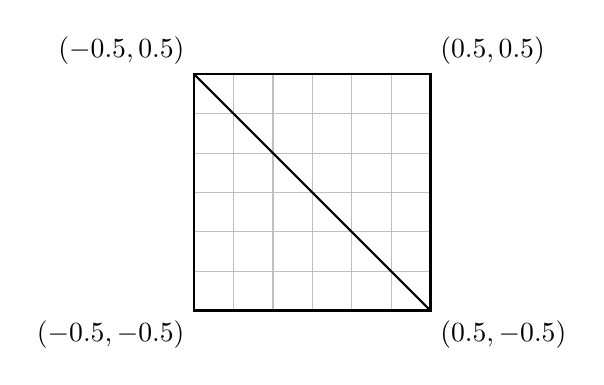
\begin{tikzpicture}[baseline={([yshift=-1em] current bounding box.north)}]
                % Grid lines
                \draw[step=0.5,lightgray,thin] (-1.5, -1.5) grid (1.5, 1.5);

                % Window edges
                \draw[thick] (-1.5, -1.5) -- (-1.5, 1.5) -- (1.5, 1.5) -- (1.5, -1.5) -- cycle;
                \draw[thick] (-1.5, 1.5) -- (1.5, -1.5);

                % Coordinates
                \draw (-1.5, -1.5) node[below left]{$\left(-0.5, -0.5\right)$};
                \draw (-1.5, 1.5) node[above left]{$\left(-0.5, 0.5\right)$};
                \draw (1.5, 1.5) node[above right]{$\left(0.5, 0.5\right)$};
                \draw (1.5, -1.5) node[below right]{$\left(0.5, -0.5\right)$};
            \end{tikzpicture}
            \item The naive way to draw this square would be to draw two triangles by specifying six vertices. Two of
                the vertices would be repeated
            \item The better way would be to list the four vertices in the square and use an element buffer object
        \end{itemize}
    \end{itemize}
\end{frame}

\begin{frame}[fragile]{Element Buffer Objects}
    \begin{itemize}
        \item To create an element buffer use {\color{blue}\verb"glGenBuffers"}
        \item Program could consist of multiple different element buffers. To make an element buffer active use
            {\color{blue}\verb"glBindBuffer"}
        \item Element data is defined as a list of integer indices
 \begin{minted}{c++}
    float vertices[] = {-0.5f, -0.5f, 0.0f,
                         0.5f, -0.5f, 0.0f,
                         0.5f,  0.5f, 0.0f,
                        -0.5f,  0.5f, 0.0f };
    unsigned int indices[] = {0, 1, 3,
                              1, 2, 3 };
 \end{minted}
        \item To copy index data to GPU memory use {\color{blue}\verb"glBufferData"}
        \item To draw an element buffer use {\color{blue}\verb"glDrawElements"}
        \item Vertex arrays will also track element buffers
    \end{itemize}
\end{frame}

\end{document}
